\chapter{Evaluation}\label{ch:evaluation}

Die in Kapitel~\ref{ch:implementation} entstandene Software wurde im Verlauf dieser Arbeit einer umfangreichen Evaluierungsphase unterzogen.
Dadurch konnten individuelle Abläufe ermöglicht, unvorhergesehene Benutzerinteraktionen erfasst und ergonomische Bedienbarkeit sichergestellt werden.
In diesem Kapitel werden drei Anwendungsfälle betrachtet, in denen die Werkzeuge fulib.org und fulibFeedback verwendet wurden.
Dabei handelt es sich um drei Veranstaltungen der Universität Kassel aus dem Sommer- bis Wintersemester 2021 bis 2022.
In Abschnitt~\ref{sec:pm-2021-2022} wird zunächst die Veranstaltung \ac{pm}\footnote{
    Fachgebiet Softwaretechnik, Prof.\ Dr.\ Albert Zündorf.
} des Wintersemesters 2021/22 betrachtet.
Die Abschnitte~\ref{sec:algods-2021} und~\ref{sec:einfinf-2021-2022} bieten daraufhin Einblicke in die Veranstaltungen "Algorithmen und Datenstrukturen"\footnote{
    Fachgebiet Programmiersprachen/-Methodik, Prof.\ Dr.\ Claudia Fohry.\label{fn:fg-plm}
} im Sommersemester 2021 und "Einführung in die Informatik"\footref{fn:fg-plm} im Wintersemester 2021/22.

\todo{
    Referenzen:
    Eingewöhnungszeit~\ref{subsec:grading}.
}

\section{\acl{pm}}\label{sec:pm-2021-2022}

Die Veranstaltung \ac{pm} stellt die größten Teil der Evaluation dar.
Sie umfasste insgesamt elf Aufgabenblätter und ein Abschlussprojekt, welche von bis zu 125 Studierenden bearbeitet und bis zu sechs Personen mit fulib.org und fulibFeedback bewertet wurden.
Dabei sind individuelle Anmerkungen sowie eine große Anzahl von Metriken in Form der Statistik entstanden.
In diesem Abschnitt werden einige Ansichten der Benutzer erläutert (Abschnitt~\ref{subsec:user-feedback}) und die Rohdaten der Statistik erfasst (Abschnitt~\ref{subsec:pm-metrics}).
Des Weiteren wird erläutert, welche Erfahrung mit den Werkzeugen zu Anpassungen der Aufgabenstellungen und Bewertungskriterien geführt haben, um den Ablauf der Bewertung zu optimieren (Abschnitt~\ref{subsec:pm-adaptations}).
Da sich die Beobachtungen und Metriken stets auf einzelne Übungsblätter beziehen, ist es an dieser Stelle lohnenswert, die elf \acp{ha} kurz zu beschreiben.

\begin{description}
    \item[\ac{ha}1] führt die Versionskontrolle mit Git ein, festigt den Unterschied zwischen den Konzepten "Abstrakt" und "Konkret" und führt Szenarien ein.\footnote{
        \url{https://seblog.cs.uni-kassel.de/wp-content/uploads/2021/10/PMWS2122_HA1.pdf}
    }
    \item[\ac{ha}2] beschäftigt sich mit Objekt- und Klassendiagrammen, die aus gegebenen Szenarien abgeleitet werden sollen.\footnote{
        \url{https://seblog.cs.uni-kassel.de/wp-content/uploads/2021/11/PMWS2122_HA2.pdf}
    }
    \item[\ac{ha}3] erwartet die händische Implementierung eines Datenmodells mit besonderem Augenmerk auf die korrekte Sicherstellung von referentieller Integrität.
    Einige prüfende Tests sind vorgegeben, ein weiterer muss selbst implementiert werden.\footnote{
        \url{https://seblog.cs.uni-kassel.de/wp-content/uploads/2021/11/PM2022_Hausaufgabe03.pdf}
    }
    \item[\ac{ha}4] führt fulib als Werkzeug zur Datenmodell-Generierung ein und ersetzt damit die händische Implementierung von \ac{ha}3.
    Darauf aufbauend soll erste Logik zur Initialisierung eines Spiels implementiert und getestet werden.\footnote{
        \url{https://seblog.cs.uni-kassel.de/wp-content/uploads/2021/11/PM_2122_Hausaufgabe04.pdf}
    }
    \item[\ac{ha}5] übt Design und Planung von Benutzeroberflächen in Form von Wireframes.
    Davon unabhängig wird das Test-First-Prinzip anhand von weiterer Spiellogik erprobt.\footnote{
        \url{https://seblog.cs.uni-kassel.de/wp-content/uploads/2021/12/PM_2022_Hausaufgabe05.pdf}
    }
    \item[\ac{ha}6] erwartet, dass die zuvor erstellten Oberflächendesigns mit \acp{fxml}\footnote{
        \ac{xml}-ähnliche Beschreibung von Oberflächen für das JavaFX-Framework.
    } umgesetzt und mit JavaFX zu einer ausführbaren Anwendung gemacht werden.
    Deren Oberfläche soll mit der TestFX-Bibliothek getestet werden.\footnote{
        \url{https://seblog.cs.uni-kassel.de/wp-content/uploads/2021/12/PM_2021_Hausaufgabe06.pdf}
    }
    \item[\ac{ha}7] beinhaltet die weitere Implementierung von Spiellogik, die dynamische Umsetzung der Oberfläche mit Controllern und zugehörige Tests.\footnote{
        \url{https://seblog.cs.uni-kassel.de/wp-content/uploads/2022/01/PM_2022_Hausaufgabe07.pdf}
    }
    \item[\ac{ha}8] verknüpft Modell und Oberfläche und hält diese bei jeder Änderung synchron, implementiert die verbleibende Spiellogik und testet den kritischen Pfad des fertigen Spiels.\footnote{
        \url{https://seblog.cs.uni-kassel.de/wp-content/uploads/2022/01/PM_2022_Hausaufgabe08.pdf}
    }
    \item[\ac{ha}9] beginnt ein neues Projekt, das initialisiert und mit einer einfachen Oberfläche versehen werden soll.\footnote{
        \url{https://seblog.cs.uni-kassel.de/wp-content/uploads/2022/01/PM_2022_Hausaufgabe09.pdf}
    }
    \item[\ac{ha}10] erweitert das neue Projekt um Serveranbindung mit \ac{rest} und dynamische Änderung der Oberfläche, um einen einfachen Chat zu ermöglichen.\footnote{
        \url{https://seblog.cs.uni-kassel.de/wp-content/uploads/2022/02/PM_WS2122_Hausaufgabe10.pdf}
    }
    \item[\ac{ha}11] ersetzt die \ac{rest}-Anbindung der vorherigen Hausaufgabe mit einer WebSocket-Schnittstelle.
    Darüber hinaus wird einfache Speicherung von Einstellungen mit \ac{json}-Dateien eingeführt.\footnote{
        \url{https://seblog.cs.uni-kassel.de/wp-content/uploads/2022/02/PM_2122_Hausaufgabe11.pdf}
    }
\end{description}

\subsection{Benutzer-Anmerkungen}\label{subsec:user-feedback}

Während der Testphase der Werkzeuge in \ac{pm} wurden die Bewertenden gebeten, nach jeder Hausaufgabe eine kurze Rückmeldung zu geben.
Diese konnte generelle Bemerkungen, Anfragen für neue Features, Verbesserungsvorschläge und kurze Fehlerberichte beinhalten.
Alle Rückmeldungen wurden in einem öffentlichen Issue\footnote{
    \url{https://github.com/fujaba/fulib.org/issues/196}
} auf GitHub gesammelt.
Nachfolgend werden einige der wichtigsten Erkenntnisse daraus beschrieben, da sie maßgeblich zu der Entwicklung von fulib.org und fulibFeedback beigetragen haben.

\subsubsection{Auswahl von Codeabschnitten}

Die wichtigste Erkenntnis aus den Benutzeranmerkungen war die Art und Weise, wie Codeabschnitte ausgewählt werden.
Der Ablauf, der in Abschnitt~\ref{subsec:choosing-code-snippets} beschrieben wurde und beide Werkzeuge symbiotisch kombiniert, wurde erst in einer späteren Version von fulibFeedback eingeführt.
Zuvor wurde die gesamte Bewertung von Code allein mit fulibFeedback gemacht.
Mittels Code Actions des \ac{lsp} wurde ein Menü angezeigt, das alle Teilaufgaben baumförmig anzeigte.
Die Aktivierung eines Menüeintrags hat dazu geführt, das über dem ausgewählten Quellcode ein Kommentar eingefügt wurde, in dem Punktzahl und Remark eingegeben werden konnten.
In diesem Kommentar konnten zwei Code Actions verwendet werden, um die Bewertung zu erstellen.
Diese Vorgehensweise hatte einige erheblich Nachteile:

\begin{itemize}
    \item Das Menü, das die Teilaufgaben anzeigte, konnte bei einer großen Anzahl von Teilaufgaben unübersichtlich werden und teilweise die Bildschirmhöhe überschreiten.
    Dies hat insbesondere die Effizienz eingeschränkt, da einige Zeit zum Suchen der nächsten unbewerteten Teilaufgabe notwendig war.
    \item Der automatisch erstellte Kommentar enthielt nur die \ac{id} der zuvor ausgewählten Teilaufgaben, aber nicht deren Beschreibung.
    Es kam vor, dass Bewertende versehentlich die falsche Teilaufgabe auswählten und dies nicht bemerkten, bevor die Bewertung erstellt wurde.
    \item Generell erforderte der automatisch erstellte Kommentar einen erheblichen Programmieraufwand seitens des Language Servers.
    Dies ist der Einschränkung des \ac{lsp} verschuldet, keine Möglichkeit zu bieten, als Teil einer Code Action den Benutzer des Editors nach einer Eingabe zu Frage.
    Wäre dies möglich, hätten Remark und Punktzahl beispielsweise über ein Prompt-Dialog erfragt werden können.
    Die hinzugefügten Kommentarzeilen erwiesen sich besonders als Problem, indem sie die darunterliegenden Zeilennummern verschoben, obwohl diese für die Hinterlegung von Codeabschnitten und für die Anzeige des Feedbacks auf GitHub relevant sind.
    \item Der Ablauf erlaubte nicht die Auswahl mehrere Codeabschnitte als Teil einer Bewertung in einem Schritt.
    Es war notwendig, zuerst einen Abschnitt auszuwählen, eine Bewertung zu erstellen, einen weiteren Abschnitt auszuwählen, und zuletzt die Bewertung zu bearbeiten.
    Dies erforderte erheblichen Aufwand bei der korrekten Implementierung von Code Search.
    Bewertungen von anderen Lösungen, die anhand des ersten Codeabschnitts automatisch erstellt wurden, mussten wieder angepasst oder \ac{ggf} gelöscht werden, falls der zweite Codeabschnitt in der Lösung nicht gefunden wurde.
    Damit verbundene Probleme haben sich besonders in \ac{ha}3 von \ac{pm} manifestiert.
\end{itemize}

Generell erwies sich diese Art der Bewertung als sehr umständlich für die Bewertenden.
Die Einführung des neuen Ablaufs aus Abschnitt~\ref{subsec:choosing-code-snippets} konnte die Implementierung der fulibFeedback-Erweiterung deutlich vereinfachen, ermöglichte neue Verbesserungen und Hilfestellungen in der fulib.org-Oberfläche und wurde von den Benutzern positiv empfangen.

\subsubsection{Benutzerfehler mit Code Search}

Die Bewertung einer großen Anzahl von Studierenden kann dazu führen, dass Fehler von den Bewertenden gemacht werden.
Dies hat sich während der Evaluationsphase in \ac{pm} zunehmend gezeigt und besonders bemerkbar gemacht, da fehlerhafte Bewertungen von einem Bewertenden auf Abgaben eines anderen von Code Search übertragen wurden.
Bei groben Fehlern führte dies dazu, dass vermeintlich bewertete Teilaufgaben nochmal überprüft werden mussten, was zusätzlichen Zeitaufwand erforderte.
Das Problem machte sich besonders in \ac{ha}7 von \ac{pm} bemerkbar\footnote{
    \url{https://github.com/fujaba/fulib.org/issues/196\#issuecomment-1022086613}
}.
Hauptursache war die Auswahl von Codeabschnitten, welche nicht eindeutig waren und unzureichenden Kontexts enthielten.
Aus diesem Grund wurden die in Abschnitt~\ref{subsec:choosing-code-snippets}, Abbildungen~\ref{fig:fulibFeedback-snippet-bad} und~\ref{fig:fulibFeedback-snippet-worst} dargestellten Informationstexte eingefügt, welche die Anzahl der von Code Search gefundenen Ergebnisse anzeigen und die Spezifität der Codeabschnitte einschätzen.
Dies erwies sich als nützlich genug, um die Benutzerfehler zu reduzieren.
Da es sich nur um eine Hilfestellung handelt, können erfahrene Benutzer dennoch Code auswählen, der nicht eindeutig ist, sofern dies als akzeptabel befunden wird.

\subsubsection{Sonstige \acl{qol}-Verbesserungen}

Dank dem ausführlichen Feedback der Betreuenden konnte neben den zuvor beschriebenen größeren Änderungen auch eine Reihe von kleinen \ac{qol}-Verbesserungen umgesetzt werden.
Hauptsächlich sind diese in Teilen der fulib.org-Oberfläche angesiedelt, die am häufigsten verwendet werden, darunter insbesondere das Bewertungs-Modalfenster (Abbildung~\ref{fig:evaluation-modal}).
Dort wurden beispielsweise die Buttons zum schnellen Einstellen der Punktzahl hinzugefügt, da häufig die Angabe der Punktzahl vergessen wurde und das Zahlenfeld schwerer zu bedienen war.
Die Möglichkeit zum Erweitern des Remark-Felds auf mehrere Zeilen ist entstanden, damit längere Hinweise und Fehlermeldung angegeben werden können.
Die Teilaufgaben-Beschreibung im Kopf des Modalfensters wurde hinzugefügt, da in einigen Fällen vergessen wurde, welche Teilaufgabe zuvor ausgewählt wurde.
Für Code Search wurde ein Banner hinzugefügt, das bei Original-Bewertungen die Anzahl der automatisch erstellten Bewertungen anzeigt, und bei letzteren einen Link zum Original.
Zuletzt hat die relativ kleine Benutzeranzahl einige Erkenntnisse zu verschiedenen Präferenzen ergeben.
Beispielsweise wurde von einem Bewertenden nicht \ac{vsc}, sondern die Open-Source-Alternative VSCodium bevorzugt.
Dessen Anbindung führte zum Hinzufügen der Optionen in der Abgaben-Tabelle (Abbildung~\ref{fig:assignment-solutions-table}).
Dies beinhaltet auch die Auswahl zwischen den Git-Clone-Optionen \ac{ssh} und \ac{https}.
Bei den Bewertenden gab es zudem Unterschiede in der Browser-Präferenz, wodurch Fehler entdeckt werden konnten, die Browser-abhängig aufgetreten sind.

\subsection{Metriken}\label{subsec:pm-metrics}

In der Veranstaltung \ac{pm} konnten dank der integrierten Statistiken von fulib.org eine Vielzahl von Messdaten ermittelt werden.
Dieser Abschnitt beschreibt einige Metriken, die darauf basieren.

\subsubsection{Effektivität}

Die Effektivität von Code Search beschreibt den prozentualen Anteil der Bewertungen, die automatisch davon erstellt wurden.
Tabelle~\ref{tbl:pm-effectiveness} zeigt für jede Hausaufgabe die Anzahl der Bewertungen von \textbf{Code Search} und \textbf{händisch} Bewertenden sowie die spezielle Kategorie der automatisch erstellten Bewertungen, die später \textbf{bearbeitet} wurden.
Diese werden in der Spalte \textbf{Gesamt} summiert, sodass die Effektivität durch Anteil von Code Search zu Gesamt berechnet werden kann.

\begin{table}
    \centering
    \caption{Bewertungen und Effektivität der \ac{pm}-Hausaufgaben}
    \begin{tabular}{|l|l|l|l|l|l|}
    \hline
        HA  & Code Search & Bearbeitet & Händisch & Gesamt & Effektivität  \\ \hline
        1  & 0 & 0 & 120 & 120 & 0\%  \\ \hline
        2  & 0 & 0 & 368 & 368 & 0\%  \\ \hline
        3  & 707 & 20 & 506 & 1233 & 57\%  \\ \hline
        4  & 3287 & 6 & 445 & 3738 & 88\%  \\ \hline
        5  & 0 & 0 & 591 & 591 & 0\%  \\ \hline
        6  & 4269 & 5 & 981 & 5255 & 81\%  \\ \hline
        7  & 2719 & 13 & 2154 & 4886 & 56\%  \\ \hline
        8  & 2081 & 1 & 1419 & 3501 & 59\%  \\ \hline
        9  & 2045 & 0 & 567 & 2612 & 78\%  \\ \hline
        10  & \multicolumn{5}{c}{\todo{}}  \\ \hline
        11  & \multicolumn{5}{c}{\todo{}}  \\ \hline
    \end{tabular}
    \label{tbl:pm-effectiveness}
\end{table}

In Abbildung~\ref{fig:pm-effectiveness} sind die relativen Verhältnisse der drei Kategorien graphisch dargestellt, um mögliche Tendenzen oder Muster ersichtlich zu machen.

\begin{figure}
    \centering
    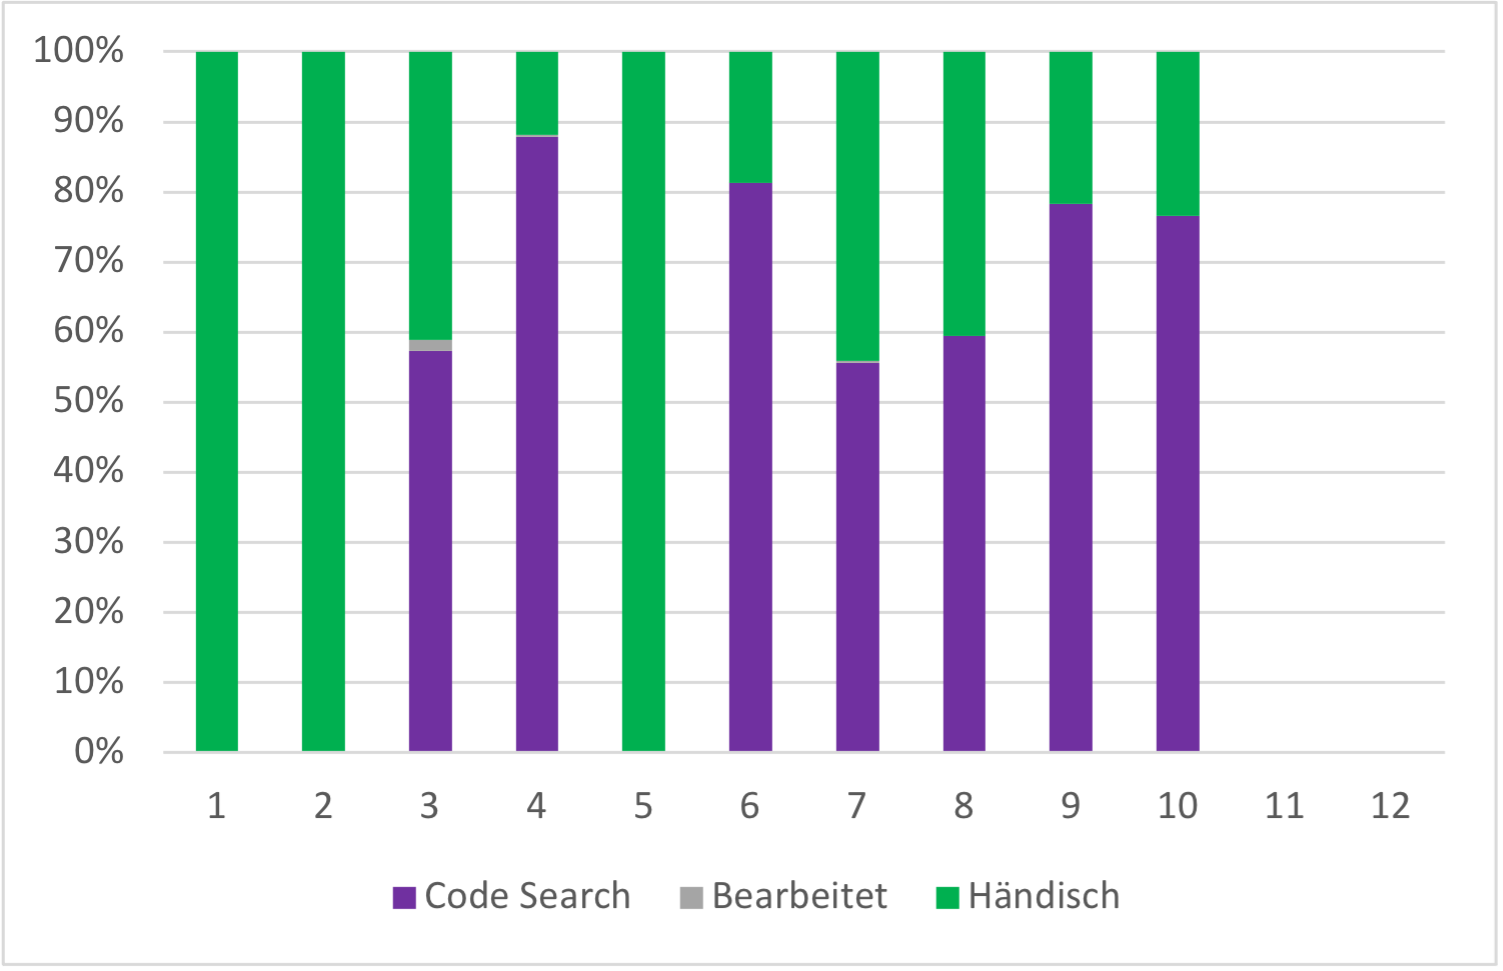
\includegraphics[width=0.6\textwidth]{graphs/pm-effectiveness}
    \caption{Effektivität der \ac{pm}-Hausaufgaben}
    \label{fig:pm-effectiveness}
\end{figure}

\todo{
    Vergleich aller Hausaufgaben.
    Wichtigste Metriken: Anteil Code Search, Zeit bewertet, Zeit gespart, Punktzahl vs Bewertungsanzahl.
    Besonderheiten bei Tasks.
}

\subsection{Anpassungen}\label{subsec:pm-adaptations}

Im Verlauf des Übungsbetriebs von \ac{pm} wurde deutlich, dass einige Anpassungen an der Aufgabenstellung zu besseren Ergebnissen mit Code Search führen können.
Es liegt nahe, dass die exakte Suche von Code Search genau dann weniger Ergebnisse erzielt, wenn Studierende eine große Vielfalt von unterschiedlichem Code abgeben.
Folglich kann die Effektivität gesteigert werden, wenn die Aufgabenstellung zur Abgabe von weniger unterschiedlichem Code verleitet.
In diesem Abschnitt werden einige Möglichkeiten zur Optimierung, die in der Veranstaltung ausprobiert wurden und sich ergeben haben, beschrieben.
Dafür ist es zunächst sinnvoll, einige Kategorien zu definieren, in denen Varianten von Quellcode fallen können, welche die Effektivität von Code Search verringern.

\begin{description}
    \item[Einrückung und sonstige Formatierung.]
    Dies umfasst die Einrückung von Quellcode mit Tabs oder Leerzeichen sowie die sonstige Platzierung von Leerzeichen um Klammern, Symbole und Bezeichnern
    Sie kann sich abhängig von den Einstellungen der \ac{ide} der Studierenden unterscheiden.
    \item[Kommentare.]
    Kommentare verhalten sich ähnlich wie Leerzeichen und Einrückung insofern, dass sie keinen Einfluss auf die Semantik von Quellcode haben.
    Es liegt nahe, diese bei der Textsuche zu ignorieren.
    \item[Benennung.]
    Eine naheliegende Ursache von Varianten ist die unterschiedliche Benennung von Bezeichnern.
    Dies umfasst Klassen, Attribute, Methoden, Parameter und lokale Variablen.
    Die Benennung folgt meist einem bestimmten Muster abhängig vom Typ:
    \code{int}-Variablen werden häufig mit Buchstaben wie \code{i}, \code{j}, \code{x} oder \code{n} benannt.
    \code{String}s werden häufig nach ihrer Rolle benannt, beispielsweise \code{name}, \code{phase}, seltener generisch wie \code{x} oder \code{value}.\footnote{
        Bei einer Analyse der Methode \code{setPhase(String)} aus Aufgabenblatt 3 ergab sich folgende Verteilung des Parameternamens:
        112 mal \code{phase}, zwei mal \code{value}, je ein mal \code{newPhase}, \code{phrase}\sic, \code{sus} und \code{x}.\label{fn:setPhase}
    }
    Objekte folgen häufig dem gleichen Muster der Benennung nach ihrer Rolle.\footnote{
        Der Parameter der Methode \code{setWinner(Player)} aus Aufgabenblatt 3 wurde wie folgt benannt:
        94 mal \code{winner}, elf mal \code{player}, vier mal \code{value}, drei mal \code{newWinner}, je ein mal \code{p}, \code{sus}, \code{winnePlayer}\sic und \code{x}.\label{fn:setWinner}
    }
    \item[Strukturierung.]
    Diese Kategorie beinhaltet insbesondere die Anordnung von imperativen Quellcode.
    Dazu zählen beispielsweise die Reihenfolge von unabhängigen Anweisungen, die Verschachtelung von \code{if}-Abfragen und Schleifen, die Operanden von kommutativen Operatoren wie \code{+}, \code{*}, \code{&&} oder \code{||}, bool'sche Ausdrücke und Klammersetzung.
    Wird von der Aufgabenstellung nur das Ergebnis einer Methode verlangt, die eigentliche Implementierung aber frei gelassen, sind die Variationen dieser Kategorie kaum voraussehbar.
    \item[Beispielwerte.]
    Die Kreativität bei Beispielwerten macht sich hauptsächlich in Tests bemerkbar.
    Sofern kein konkretes Szenario vorgegeben ist, das vom Test durchgeführt werden soll, sind Studierende frei in der Wahl von Namen, Zahlen und sonstigen Zeichenketten.
\end{description}

Das Problem der unterschiedlichen Einrückung und Formatierung wird bereits von Code Search gelöst, indem die Tokenisierung sämtliche Leerzeichen ignoriert und nicht in die Suche einbezieht.
Kommentare werden hingegen nicht ignoriert, da sie bei einigen Hausaufgaben hilfreich für die Einschränkung von Code Search durch Kontext waren.
Darüber hinaus haben einige Aufgabenblätter\footnote{
    Hausaufgaben 7, 8, 10 und 11.
} verlangt, dass besondere \code{TODO}-Kommentare entfernt werden.
Dies wäre mit Code Search nicht prüfbar gewesen, wenn die Kommentare wie Leerzeichen behandelt worden wären.

Die Benennung kann durch Angaben in der Aufgabenstellung standardisiert werden.
In den Programmieraufgaben der Veranstaltung waren das Datenmodell und Methodennamen vorgegeben, wodurch primär Parameter und lokale Variablen unterschiedlich benannt wurden.
Es hat sich gezeigt, dass die meisten Studierenden ähnliche Namengebungs-Strategien verfolgen\footref{fn:setPhase}~\footref{fn:setWinner} und dadurch die Effektivität nur geringfügig beeinflusst wird.
Sonstige Bezeichner, beispielsweise \acp{id} von Oberflächenelementen, wurden in den Hausaufgaben 4, 6 und 9 vorgegeben.
Abbildung~\todo{XX (Metriken)} der Metriken zeigt, dass dies mit besserer Code Search-Effektivität verbunden ist.

Für die Strukturierung hat sich im Verlauf der Veranstaltung eine unbeabsichtigte Lösung ergeben.
Vorwiegend betraf dies die Hausaufgaben 7 und 8.
Es wurden Vorlagen bereitgestellt, welche mit Kommentaren darauf hinweisen, an welchen Stellen im Code bestimmte Funktionalität implementiert werden muss.
Dies verleitete Studierende dazu, ähnlich strukturierte Lösungen abzugeben.
Insbesondere beeinflusste dies die Schachtelung von \code{if}-Anweisungen und Schleifen sowie die Reihenfolge von imperativen Code.
Dennoch entstanden Variationen durch das optionale \code{this}\footnote{
    Dieses Sprachkonstrukt von Java kann für qualifizierte Attributzugriffe und Methodenaufrufe mit dem aktuellen Objekt verwendet werden, ist aber meist nicht notwendig.
}, Klammersetzung, bool'sche Operationen und kommutative Operanden.
Aus diesem Grund ist eine große Bandbreite an Effektivitäts-Werten für Teilaufgaben dieser Hausaufgaben entstanden, welche sich jedoch insgesamt zu einem mittelmäßigen Ergebnis ausgleichen.

Das Problem der Beispielwerte in Tests hat sich über alle Übungsblätter mit solchen bemerkbar gemacht.
Dort wurden teilweise keine Ergebnisse von Code Search gefunden und somit keine Zeit eingespart.
\ac{ha}5 stellt dafür ein Extrembeispiel dar, weil sich diese inhaltlich mit dem Test-First-Prinzip befasste und dadurch die Tests einen Großteil der Punkte beisteuerten.
Weiterhin wurde in diesem Aufgabenblatt verlangt, Mockups anzufertigen, welche keinen Code benötigen und damit nicht für Code Search geeignet sind.

\section{Algorithmen und Datenstrukturen}\label{sec:algods-2021}

\todo{
    Keine Bewerter, nur Betrachten der Daten.
    Statistiken.
}

\section{Einführung in die Informatik}\label{sec:einfinf-2021-2022}

\todo{
    Erfahrungsbericht, User Feedback.
}
